\documentclass[10pt,twocolumn,letterpaper]{article}

\usepackage{cvpr}
\usepackage{times}
\usepackage{epsfig}
\usepackage{graphicx}
\usepackage{amsmath}
\usepackage{amssymb}
\usepackage[italian]{babel}

\usepackage{url}
\usepackage{listings}
\usepackage{xcolor}

\lstset{
  language=Python,
  basicstyle=\ttfamily\small,
  keywordstyle=\color{blue},
  commentstyle=\color{green!50!black},
  stringstyle=\color{red},
  numbers=left,
  numberstyle=\tiny\color{gray},
  breaklines=true,
  frame=L,
  captionpos=b,     % Sposta la caption in basso
  basicstyle=\ttfamily\small, % Opzionale: un font monospace più elegante
  breaklines=true
}

% Include other packages here, before hyperref.

% If you comment hyperref and then uncomment it, you should delete
% egpaper.aux before re-running latex.  (Or just hit 'q' on the first latex
% run, let it finish, and you should be clear).
%\usepackage[pagebackref=true,breaklinks=true,letterpaper=true,colorlinks,bookmarks=false]{hyperref}

\cvprfinalcopy % *** Uncomment this line for the final submission

\def\cvprPaperID{****} % *** Enter the CVPR Paper ID here
\def\httilde{\mbox{\tt\raisebox{-.5ex}{\symbol{126}}}}

% Pages are numbered in submission mode, and unnumbered in camera-ready
\ifcvprfinal\pagestyle{empty}\fi
\begin{document}

%%%%%%%%% TITLE
\title{Estrazione di N-Grams: Confronto fra la versione sequenziale e parallela implementate in Python}

\author{Mattia Baroncelli\\
7166468\\
{\tt\small mattia.baroncelli@edu.unifi.it}
% For a paper whose authors are all at the same institution,
% omit the following lines up until the closing ``}''.
% Additional authors and addresses can be added with ``\and'',
% just like the second author.
% To save space, use either the email address or home page, not both
}

\maketitle
\thispagestyle{empty}

%%%%%%%%% ABSTRACT
\begin{abstract}
   Il progetto si concentra sull'implementazione di un algoritmo che consenta di contare le istanze di bi-gram e tri-gram all'interno di un testo. Questo inteso sia come composizione di caratteri, che come composizione di parole. E' chiaro, a partire dalla natura del progetto, come all'aumentare della dimensione del file dato in input, i tempi di esecuzione si dilatino notevolemnte.
   Lo scopo principale del progetto pertanto è quella di implementare una versione parallela dell'algoritmo, che vada a velocizzare il processo. La soluzione verrò data sia tramite la libreria \textit{Multiprocessing} che utilizzando \textit{JobLib}.
\end{abstract}

%%%%%%%%% BODY TEXT
\noindent\textbf{Future Distribution Permission}\\
\indent The author(s) of this report give permission for this document to be distributed to Unifi-affiliated students taking future courses.

\section{Introduzione}

L'obiettivo principale del progetto è quello di creare un algoritmo che ci permetta di contare gli n-grams presenti in un file dato in input. Gli n-grams sono sequenze di n caratteri (o parole) consecutive che si riscontrano all'interno del testo. In particolare in questo progetto ci concentreremo sulla ricerca dei bi-gram e dei tri-gram (ossia le sequenze con n=2 e n=3). Nel caso dei bi-gram quindi l'algoritmo andrà a ricercare tutte le coppie di caratteri vicine all'interno del testo e successivamente conterà le occorrenze delle coppie all'interno del testo.
Una delle maggiori criticità dell'algoritmo si presenta quando la dimensione del testo risulta essere molto grande, poichè il processo di contare le occorrenze all'interno del testo può durare molto tempo. Con lo scopo di superare queste limitazioni abbiamo implementato alcune versioni parallele dell'algoritmo, che riescono a suddividere le operazioni fra i vari core, andando a ridurre i tempi di esecuzione.
Il processo di parallelizzazione è stato fatto usando Python; in particolare le due librerie \textit{Multiprocessing} e \textit{JobLib}. Andremo quindi a valutare quanto l'impatto della parallelizzazione migliori le prestazioni del conteggio degli n-grams.

\begin{figure}[t]
\begin{center}
   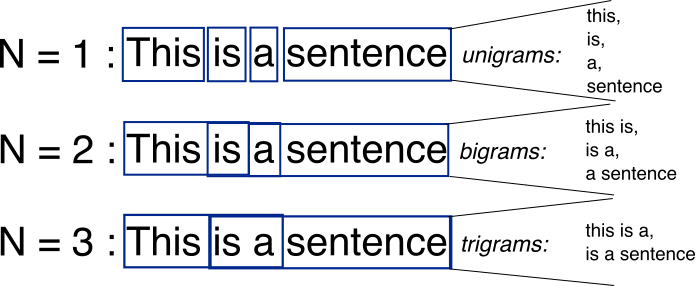
\includegraphics[width=0.9\linewidth]{img1.png}
\end{center}
   \caption{Esempio di uni-gram, bi-gram e tri-gram.}
\label{fig:kmeans_example}
\end{figure}


%-------------------------------------------------------------------------
\section{Implementazione}
Andiamo adesso a vedere alcune fasi necessarie e scelte di implementazione del codice.
\subsection{Dataset}
Prima di iniziare a descrivere l'algoritmo è necessario procedere con una fase pregressa, ossia quella di normalizzazione del testo. Innanzitutto tutti i testi che andremo ad usare saranno in lingua inglese ed estratti da testi provenienti da \textit{Gutenberg Project}, un sito che permette l'accesso gratuito a numerosi testi della letteratura inglese in formato UTF-8. Un'ecccezione è rappresentata dal dataset \textit{text8 dataset} che è una collezione della dimensione di 100 MB, di testo estratto da Wikipedia. Per poter avere a disposizione un file di dimensione a piacere abbiamo creato uno script \lstinline{create_large_corpus} che permette di copiare il testo contenuto in un file per un numero desiderato di volte all'interno di un altro file. I file a cui si fa riferimento sono in formato \textit{.txt} e non sono presenti all'interno del repository, ma sono facilmente reperibili.
\subsection{Normalizzazione}
Una volta estratto il testo questo viene sottoposto ad un processo di normalizzazione, in modo da ridurre la dimensione del dizionario complessivo e rendere più facile l'individuazione degli n-grams, questo viene fatto tramite le funzioni \lstinline{clean_chars} e \lstinline{clean_words}.
Nello specifico queste eliminano tutti i caratteri in maiuscolo, rimuovono la punteggiatura e nel caso dei caratteri eliminano tutti gli spazi fra parole diverse.

\subsection{Struttura dati Counter}
Come abbiamo visto lo scopo principale del progetto è contare le occorrenze degli n-grams, ed è importante notare come nel caso di testo dell'ordine dei GB è necessaria una struttura dati che ci permetta di memorizzare le istanze presenti nel dizionario in modo efficiente. Per questo all'interno del progetto viene usata la struttura dati \lstinline{Counter}, questa è una Hash Map, che permette di accedere allo slot di memoria relativo ad un n-gram, senza dover scorrere la lista di tutti gli n-gram. Inoltre vedremo che questa struttura dati ci permetterà di sommare con semplicità i contatori parziali della versione parallela del codice.
%-------------------------------------------------------------------------

\section{Codice}
In questa sezione andiamo a vedere le diverse versioni del codice che implementa il conteggio degli n-grams. I task principali sono due, ossia: il conteggio di n-gram di caratteri e il conteggio di n-gram di parole. Poichè il codice per svolgere i due task è molto simile, e varia principalmente nella fase di preprocessing, verrà mostrato solo quello riguardante i caratteri.

\subsection{Versione sequenziale}
Iniziamo l'analisi con la versione sequenziale dell'algoritmo.
Il codice per la versione sequenziale è contenuto nel file \lstinline{sequential_counter} ed è formato da due fasi principali:
\begin{itemize}
   \item Estrazione degli n-grams
   \item Conteggio delle occorrenze all'interno del testo
\end{itemize}
Di seguito vediamo le funzioni che svolgono questo compito, nel caso del conteggio dei bigrams formati da caratteri vicini.
\begin{lstlisting}[caption={Estrazione degli n-grams sequenziale.}]
def get_ngrams(seq, n):
    limite = len(seq) - n + 1
    for i in range(limite):
        sl = seq[i : i+n]
        yield tuple(sl)
\end{lstlisting}

\begin{lstlisting}[caption={Conteggio dei bi-grams}]
def compute_bigrams(chars):
    b_chars = Counter(get_ngrams(chars, 2))
    return b_chars
\end{lstlisting}

La prima funzione prende in input il testo che ha già subito la fase di preprocessing e la dimensione di n-grams desiderata (2 per i bi-grams, 3 per i tri-grams...). Poi scorrendo tutta la sequenza di testo estrae sottosequenze di caratteri lunghe quanto il parametro \textit{n}, convertendole in tuple. Successivamente tramite il costrutto "yield" restituisce l'ngram generato alla funzione \lstinline{get_ngrams} che si occupa di allocare la locazione di memoria che permette di contare le occorrenze nel caso sia un nuova n-grams, mentre aggiornerà il contatore per quelli che sono già presenti nella struttura dati.
L'uso del costrutto \lstinline{yield} è stato cruciale per quanto riguarda l'ottimizzazione del codice. Una prima soluzione era stata quella di inserire ogni n-gram trovato all'interno di una lista e poi passarla al Counter per permettere di contare le occorrenze; questo presentava problemi nel caso di corpus di dimensioni molto elevate. L'operazione di inserimento costringe a dover scorrere tutta la lista e quando il numero di n-grams è elevato, l'operazione diventa molto costosa. In questo modo invece ad ogni ciclo il codice si interrompe per passare l'n-gram alla funzione che ne andrà a fare l'hashing. Il codice sequenziale pertanto risulta semplice, ma riesce a svolgere il task senza problemi.

\subsection{Versione parallela}
Dopo aver implementato la versione sequenziale del codice vediamo adesso come è possibile passare ad una versione parallela. La versione parallela è stata sviluppata mediante due librerie diverse che abbiamo visto durante le lezioni del corso:
\begin{itemize}
   \item Multiprocessing: La libreria nativa di Python, permette di aggirare il GIL, andando a creare dei processi figli del programma originale.
   \item JobLib: Una libreria che sfrutta il backend "Loky", che permette di gestire i cali di memoria e prevenire i deadlocks. Inoltre permette di salvare grandi quantità di dati su una memoria condivisa permettendo ai processi di accedervi, evitando di clonare i dati.
\end{itemize}

Iniziamo l'analisi dal paredigma utilizato per fare il codice, ossia MapReduce. In questo approcco si divide il task in due fasi primitive denominate Map e Reduce applicate a coppie chiave-valore. Nella fase di Map, una funzione di mapping viene applicata in parallelo ad ogni split del dataset, dando in output delle coppie chiave-valore. Successivamente le coppie intermedie vengono raggruppate per chiave. Infine una funzione Reduce aggrega i risultati intermedi.
Nel caso del conteggio degli n-grams la fase di Map individua gli n-grams presenti in ogni split del dataset. Successivamente si procederà al conteggio parziale e infine la funzione Reduce andrà a sommare i risultati parziali. Il nostro obiettivo quindi è suddividere il testo totale in chunk della stessa grandezza, assegnare ogni chunk ad un core, far contare le occorrenze degli n-grams ad ogni core nel proprio chunk ed infine sommare tutti i risultati ottenuti da ogni core.

\subsubsection{Multiprocessing}
Il primo metodo usato per sviluppare la versione parallela è attraverso l'utilizzo di \textit{Multiprocessing}. Si noti che per tutte le versioni parallele il metodo \lstinline{get_ngrams} resta uguale alla versione sequenziale e lo stesso vale per le funzioni che calcolano bigrams e trigrams. Questo succede perchè il nostro approccio consiste nel dividere il testo in molteplici chunk e applicare gli stessi metodi su questi, invece che sull'intero testo.
E' necessaria pertanto delle funzioni che si occupino di queste operazioni. In particolare della creazione dei chunk e dell'assegnazione dei processi ad ogni core.
Andiamo a vedere innanzitutto la funzione che crea i chunk.

\begin{lstlisting}[caption={Creazione di chunk di testo.}]
def get_chunks(cleaned_text, num_chunks, max_ngram_size=3):
    chunk_size = len(cleaned_text) // num_chunks
    chunks = []
    overlap = max_ngram_size - 1

    for i in range(num_chunks):
        start = i * chunk_size
        if i == num_chunks - 1:
            end = len(cleaned_text)
        else:
            end = (i + 1) * chunk_size + overlap
        sl = cleaned_text[start:end]
        chunks.append(sl)
        
    return chunks
\end{lstlisting}

Il codice andrà quindi a creare dei chunk del testo completo di dimensione uguale, che andranno divisi fra i vari core. Un aspetto importante riguarda la gestione dell'overlap fra i diversi chunk. Infatti dividendo in modo netto un chunk da un altro si andranno a perdere gli n-gram i cui caratteri si trovano alcuni in un chunk e altri nel successivo. Per risolvere il problema è stato aggiunto un parametro overlap che andrà a considerare nel caso in cui ci trovassimo alla fine di un chunk anche i successivi caratteri.\par
Adesso soffermiamoci sulla porzione di codice che implementa la divisione del task fra i vari core e che fa uso di \textit{Multiprocessing}. In particolare forniamo la versione dei bigram di caratteri, il codice delle altre versioni si trova su Github ma è analogo a questo.

\begin{lstlisting}[caption={Calcolo degi n-grams con Multiprocessing.}]
def compute_bigrams_parallel(chars, num_cores):
    chunks_b = get_chunks(chars, num_chunks=num_cores, max_ngram_size=2)
    with multiprocessing.Pool(processes=num_cores) as pool:
        partial_counters_b = pool.map(process_chunk_bigrams, chunks_b)
    return sum(partial_counters_b, Counter())
\end{lstlisting}

Il codice è suddiviso in due parti principali, in linea con il paradigma Map-Reduce. Nella prima parte il file viene diviso in un numero di chunk pari al numero di cores che si vogliono usare, successivamente vengono creati \textit{numcores} processi separati e tramite la funzione \lstinline{map} viene assegnato ad ogni core un chunk e viene applicata la funzione che conta le occorrenze degli n-grams. Nella seconda parte, viene fatta la fase di Reduce, dove si andranno a sommare i contatori parziali di ogni core.

\subsubsection{JobLib}
Come altro metodo abbiamo implementato il task tramite JobLib, anche in questo caso sia per gli n-gram di caratteri che per quelli di parole. Lo scopo di questo esperimento è vedere se tramite esperimenti con dimensioni di file più grandi si notano variazioni nelle performance fra metodi diversi di parallelizzazione. In questo caso la funzione per ottenere i chunk non subisce alcuna modifica rispetto a quella illustrata prima. Andiamo quindi a vedere come avviene il conteggio degli n-grams.

\begin{lstlisting}[caption={Calcolo degi n-grams con JobLib.}]
def compute_bigrams_joblib(chars, num_cores):
    chunks_b = get_chunks(chars, num_chunks=num_cores, max_ngram_size=2)
    partial_counters_b = Parallel(n_jobs=num_cores, batch_size='auto')(
        delayed(process_chunk_bigrams)(chunk) for chunk in chunks_b
    )
    return sum(partial_counters_b, Counter())
\end{lstlisting}

Come possiamo vedere il codice scritto sfruttando \textit{JobLib} presenta una sintassi diversa rispetto a quello scritto con \textit{Multiprocessing}. La parte principale del codice è quella usata per costruire il contatore parziale, ossia \textit{Parallel}. A questa vengono indicati il numero di core e tramite il parametro \textit{batchsize} impostato ad \textit{auto} indichiamo l'ottimizzazione intelligente del carico, che vedremo risultare molto utile successivamente. Nelle parentesi seguenti viene indicato il modo con cui eseguire l'esecuzione, tramite il costrutto \textit{delayed}; questo permette di non eseguire immediatamente l'esecuzione, in modo da attendere che i processi vengano assegnati ai core.

\subsubsection{Threading}
L'ultimo metodo da analizzare è tramite \textit{Threading}, questo ho deciso di posizionarlo nel capitolo dedicato alle versioni parallele anche se vedremo che si differenzierà dagli altri due metodi. Le differenze principali con i metodi che abbiamo visto sono: che lo spazio di memoria fra i threads è condiviso, ma soprattutto è presente il meccanismo di context switching che permette ad un solo thread alla volta di svolgere il task.
Vediamo quindi come viene usato \textit{Threading} per implementare il conteggio degli n-grams, in particolare nel caso dei bi-grams.


\begin{lstlisting}[caption={Calcolo degi n-grams con JobLib.}]
def compute_bigrams_threading(chars, num_threads):
    chunks_b = get_chunks(chars, num_chunks=num_threads, max_ngram_size=2)
    res = queue.Queue()
    threads = []

    for chunk in chunks_b:
        t = threading.Thread(
            target=thread_worker, 
            args=(process_chunk_bigrams, chunk, res)
        )
        threads.append(t)
        t.start()
        
    for t in threads:
        t.join()

    partial_counters_b = []
    while not res.empty():
        partial_counters_b.append(res.get())
        
    return sum(partial_counters_b, Counter())
\end{lstlisting}

Dopo aver suddiviso il testo in chunks, è stato necessario implementare una coda condivisa, tramite \lstinline{queue.Queue()} che garantisce che non si verifichino condizioni di race condition fra threads. Successivamente si andrà a chiamare thread workers il cui unico scopo è di effettuare il conteggio e riportare il risultato all'interno della coda. Infine con il metodo join si vanno a eseguire i threads. Il codice continua con la parte di reduce che però non ho riprtato perchè poco interessante.

%-------------------------------------------------------------------------

\section{Esperimenti}
Iniziamo adesso la sezione del report che riguarda gli esperimenti effettuati, abbiamo visto come i tre diversi tipi di implementazione variano, adesso vediamo quanto queste variano a livello di prestazioni.
Gli esperimenti sono stati fatti sui seguenti testi:
\begin{itemize}
    \item Frankestein - Mary Shelley (78099 parole)
    \item Frankestein - Mary Shelley ripetuto per 50 volte (3.904.950 parole)
    \item Dataset "text8" (100 MB - 17.057.642 parole)
\end{itemize}
\subsection{N-Gram di Caratteri}
Valutiamo innanzitutto il calcolo delle occorrenze di n-gram di caratteri all'interno dei testi.
Come primo esperimento valutiamo le quattro versioni in termini di tempo di esecuzione e speedup nel caso in cui nelle versioni parallele si vadano a creare chunk tutti della stessa dimensione, ossia del numero di caratteri totali diviso il numero di core. Ed usiamo un numero di core pari a 8 in tutte le versioni.

%table (Testo x Modalità X execTime/speedup con fissi 4 core)
\begin{table}[ht]
\centering
\caption{Confronto prestazioni nel calcolo dei Bi-gram di caratteri (8 Core)}
\label{tab:performance_comparison}
\resizebox{\columnwidth}{!}{%
\begin{tabular}{|l|cc|cc|cc|}
\hline
                & \multicolumn{2}{c|}{\textbf{Frankenstein}} & \multicolumn{2}{c|}{\textbf{Frank. x50}} & \multicolumn{2}{c|}{\textbf{Text8 (100MB)}} \\
\textbf{Metodo} & Time (s) & Speedup & Time (s) & Speedup & Time (s) & Speedup \\ \hline \hline
Sequenziale     & 0.12     & -       & 5.32    & -       & 25.02    & -       \\ \hline
Threading       & 0.10     & 1.2x    & 7.09     & 0.75x   & 27.78    & 0.90x   \\ \hline
Multiprocessing & 0.22     & 0.54x   & 2.05     & 2.59x   & 11.74    & 2.13x   \\ \hline
JobLib          & 0.24     & 0.50x   & 2.24     & 2.37x   & 11.92    & 2.09x   \\ \hline
\end{tabular}%
}
\end{table}




\begin{table}[ht]
\centering
\caption{Confronto prestazioni nel calcolo dei Tri-gram di caratteri (8 Core)}
\label{tab:performance_comparison}
\resizebox{\columnwidth}{!}{%
\begin{tabular}{|l|cc|cc|cc|}
\hline
                & \multicolumn{2}{c|}{\textbf{Frankenstein}} & \multicolumn{2}{c|}{\textbf{Frank. x50}} & \multicolumn{2}{c|}{\textbf{Text8 (100MB)}} \\
\textbf{Metodo} & Time (s) & Speedup & Time (s) & Speedup & Time (s) & Speedup \\ \hline \hline
Sequenziale     & 0.15     & -       & 5.85     & -       & 32.54    & -       \\ \hline
Threading       & 0.14     & 1.07x    & 7.22     & 0.81x   & 33.06    & 0.98x   \\ \hline
Multiprocessing & 0.18     & 0.83x   & 1.92     & 3.04x   & 16.89    & 1.92x   \\ \hline
JobLib          & 0.17     & 0.88x   & 1.86     & 3,15x   & 16.47    & 1.97x   \\ \hline
\end{tabular}%
}
\end{table}


Come è possibile vedere dalle tabelle nel caso in cui viene fatto l'n-gram di caratteri, le prestazioni di entrambe le versioni parallele risultano migliori di quella sequenziale per quanto riguarda i testi lunghi. Per il solo testo di "Frankestein" le performance sono quasi uguali come tempo di esecuzione, con un leggero vantaggio della versione sequenziale. In questi casi il tempo impiegato per le operazioni di preprocessing (chunking e assegnazione) è paragonabile al tempo necessario ad eseguire il task, rendendo la parallelizzazione superflua. Possiamo notare come il task riguardante i trigram ottenga benefici migliori dalla parallelizzazione sul dataset \textit{Frankestein x50}, ma vada a perdere su \textit{Text8}, questo a prima vista può sembrare un comportamento anomalo, di cui ci concentreremo nelle prossime sezioni
E' interessante invece notare nei testi di grande dimensione che lo speedup fra le due versioni parallele dello stesso task non varia molto, e diversamente da quanto era possibile pensare all'aumentare della dimensione del dataset lo speedup non migliora; anche questo verrà analizzato in seguito. Per quanto riguarda la versione con \textit{Threading}, questa risulta essere al pari di quella sequenziale nel dataset più piccolo, ma peggiora drasticamente le performance con l'aumentare della dimensione. 

\subsection{N-Gram di Parole}
Procediamo ora con l'analisi degli esperimenti riguardanti gli n-gram di parole. Anche in questo caso ripetiamo gli stessi esperimenti di prima, non andando a variare il numero di core. 


%table (Testo x Modalità X execTime/speedup con fissi 4 core)
\begin{table}[ht]
\centering
\caption{Confronto prestazioni nel calcolo dei Bi-gram di parole (8 Core)}
\label{tab:performance_comparison}
\resizebox{\columnwidth}{!}{%
\begin{tabular}{|l|cc|cc|cc|}
\hline
                & \multicolumn{2}{c|}{\textbf{Frankenstein}} & \multicolumn{2}{c|}{\textbf{Frank. x50}} & \multicolumn{2}{c|}{\textbf{Text8 (100MB)}} \\
\textbf{Metodo} & Time (s) & Speedup & Time (s) & Speedup & Time (s) & Speedup \\ \hline \hline
Sequenziale     & 0.02     & -       & 2.43    & -       &  14.66    & -       \\ \hline
Threading       & 0.09     & 0.22x    & 2.38     & 1.02x   & 19.22    & 0.76x   \\ \hline
Multiprocessing & 0.35     & 0.05x   & 1.59     & 1.52x   & 33.10    & 0.44x   \\ \hline
JobLib          & 0.39     & 0.05x   & 1.62     & 1.5x   & 31.47    & 0.47x   \\ \hline
\end{tabular}%
}
\end{table}




\begin{table}[ht]
\centering
\caption{Confronto prestazioni nel calcolo dei Tri-gram di parole (8 Core)}
\label{tab:performance_comparison}
\resizebox{\columnwidth}{!}{%
\begin{tabular}{|l|cc|cc|cc|}
\hline
                & \multicolumn{2}{c|}{\textbf{Frankenstein}} & \multicolumn{2}{c|}{\textbf{Frank. x50}} & \multicolumn{2}{c|}{\textbf{Text8 (100MB)}} \\
\textbf{Metodo} & Time (s) & Speedup & Time (s) & Speedup & Time (s) & Speedup \\ \hline \hline
Sequenziale     & 0.03     & -       & 2.66     & -       & 15.22    & -       \\ \hline
Threading       & 0.10     & 0.30x    & 2.61     & 1.01x   & 20.57    & 0.73x   \\ \hline
Multiprocessing & 0.37     & 0.08x   & 1.78     & 1.49x   & 109.72    & 0.14x   \\ \hline
JobLib          & 0.14     & 0.21x   & 1.83     & 1.45x   & 112.03    & 0.13x   \\ \hline
\end{tabular}%
}
\end{table}

Le tabelle mostrano risultati interessanti e piuttosto inaspettati, differentemente da prima gli approcci paralleli non scalano con la dimensione del file, ma dipendono dalla dimensione del vocabolario.
Su testi piccoli (Frankestein) non ci aspettavamo grandi differenze, poichè il tempo di esecuzione dell'algoritmo è molto breve.
Nel dataset medio i due approcci paralleli superano quello sequenziale ottenendo uno speedup di circa 1.5x in entrambi i casi. Il caso più eclatante è quello che riguarda il dataset \textit{text8}. In questo scenario i metodi paralleli collassano impiegando più del doppio del tempo sui bi-gram rispetto alla versione sequenziale e quasi sette volte il tempo sui trigrammi.
Questo è dovuto a due motivi principali: in primo luogo il dataset contiene un vocabolario vastissimo, che rende il numero di n-gram totali nell'ordine dei milioni. I processi al termine del calcolo devono inviare i risultati sotto forma di dizionario al processo principale, saturando le risorse del sistema operativo. Il secondo motivo è da ritrovarsi nella parte che opera il reduce; la fase di somma infatti costringe a effettuare continui cicli di allocazione e deallocazione nella RAM. Il tutto senza dubbio è confermato dall'incremento repentino fra bi-grammi e tri-grammi. Tutto questo è confermato dal grafico in Figura \ref{fig:profiling1} estratto da una fase di profiling effettuata sul codice che estrae i bi-grams di parole.

\begin{figure}[t]
\begin{center}
   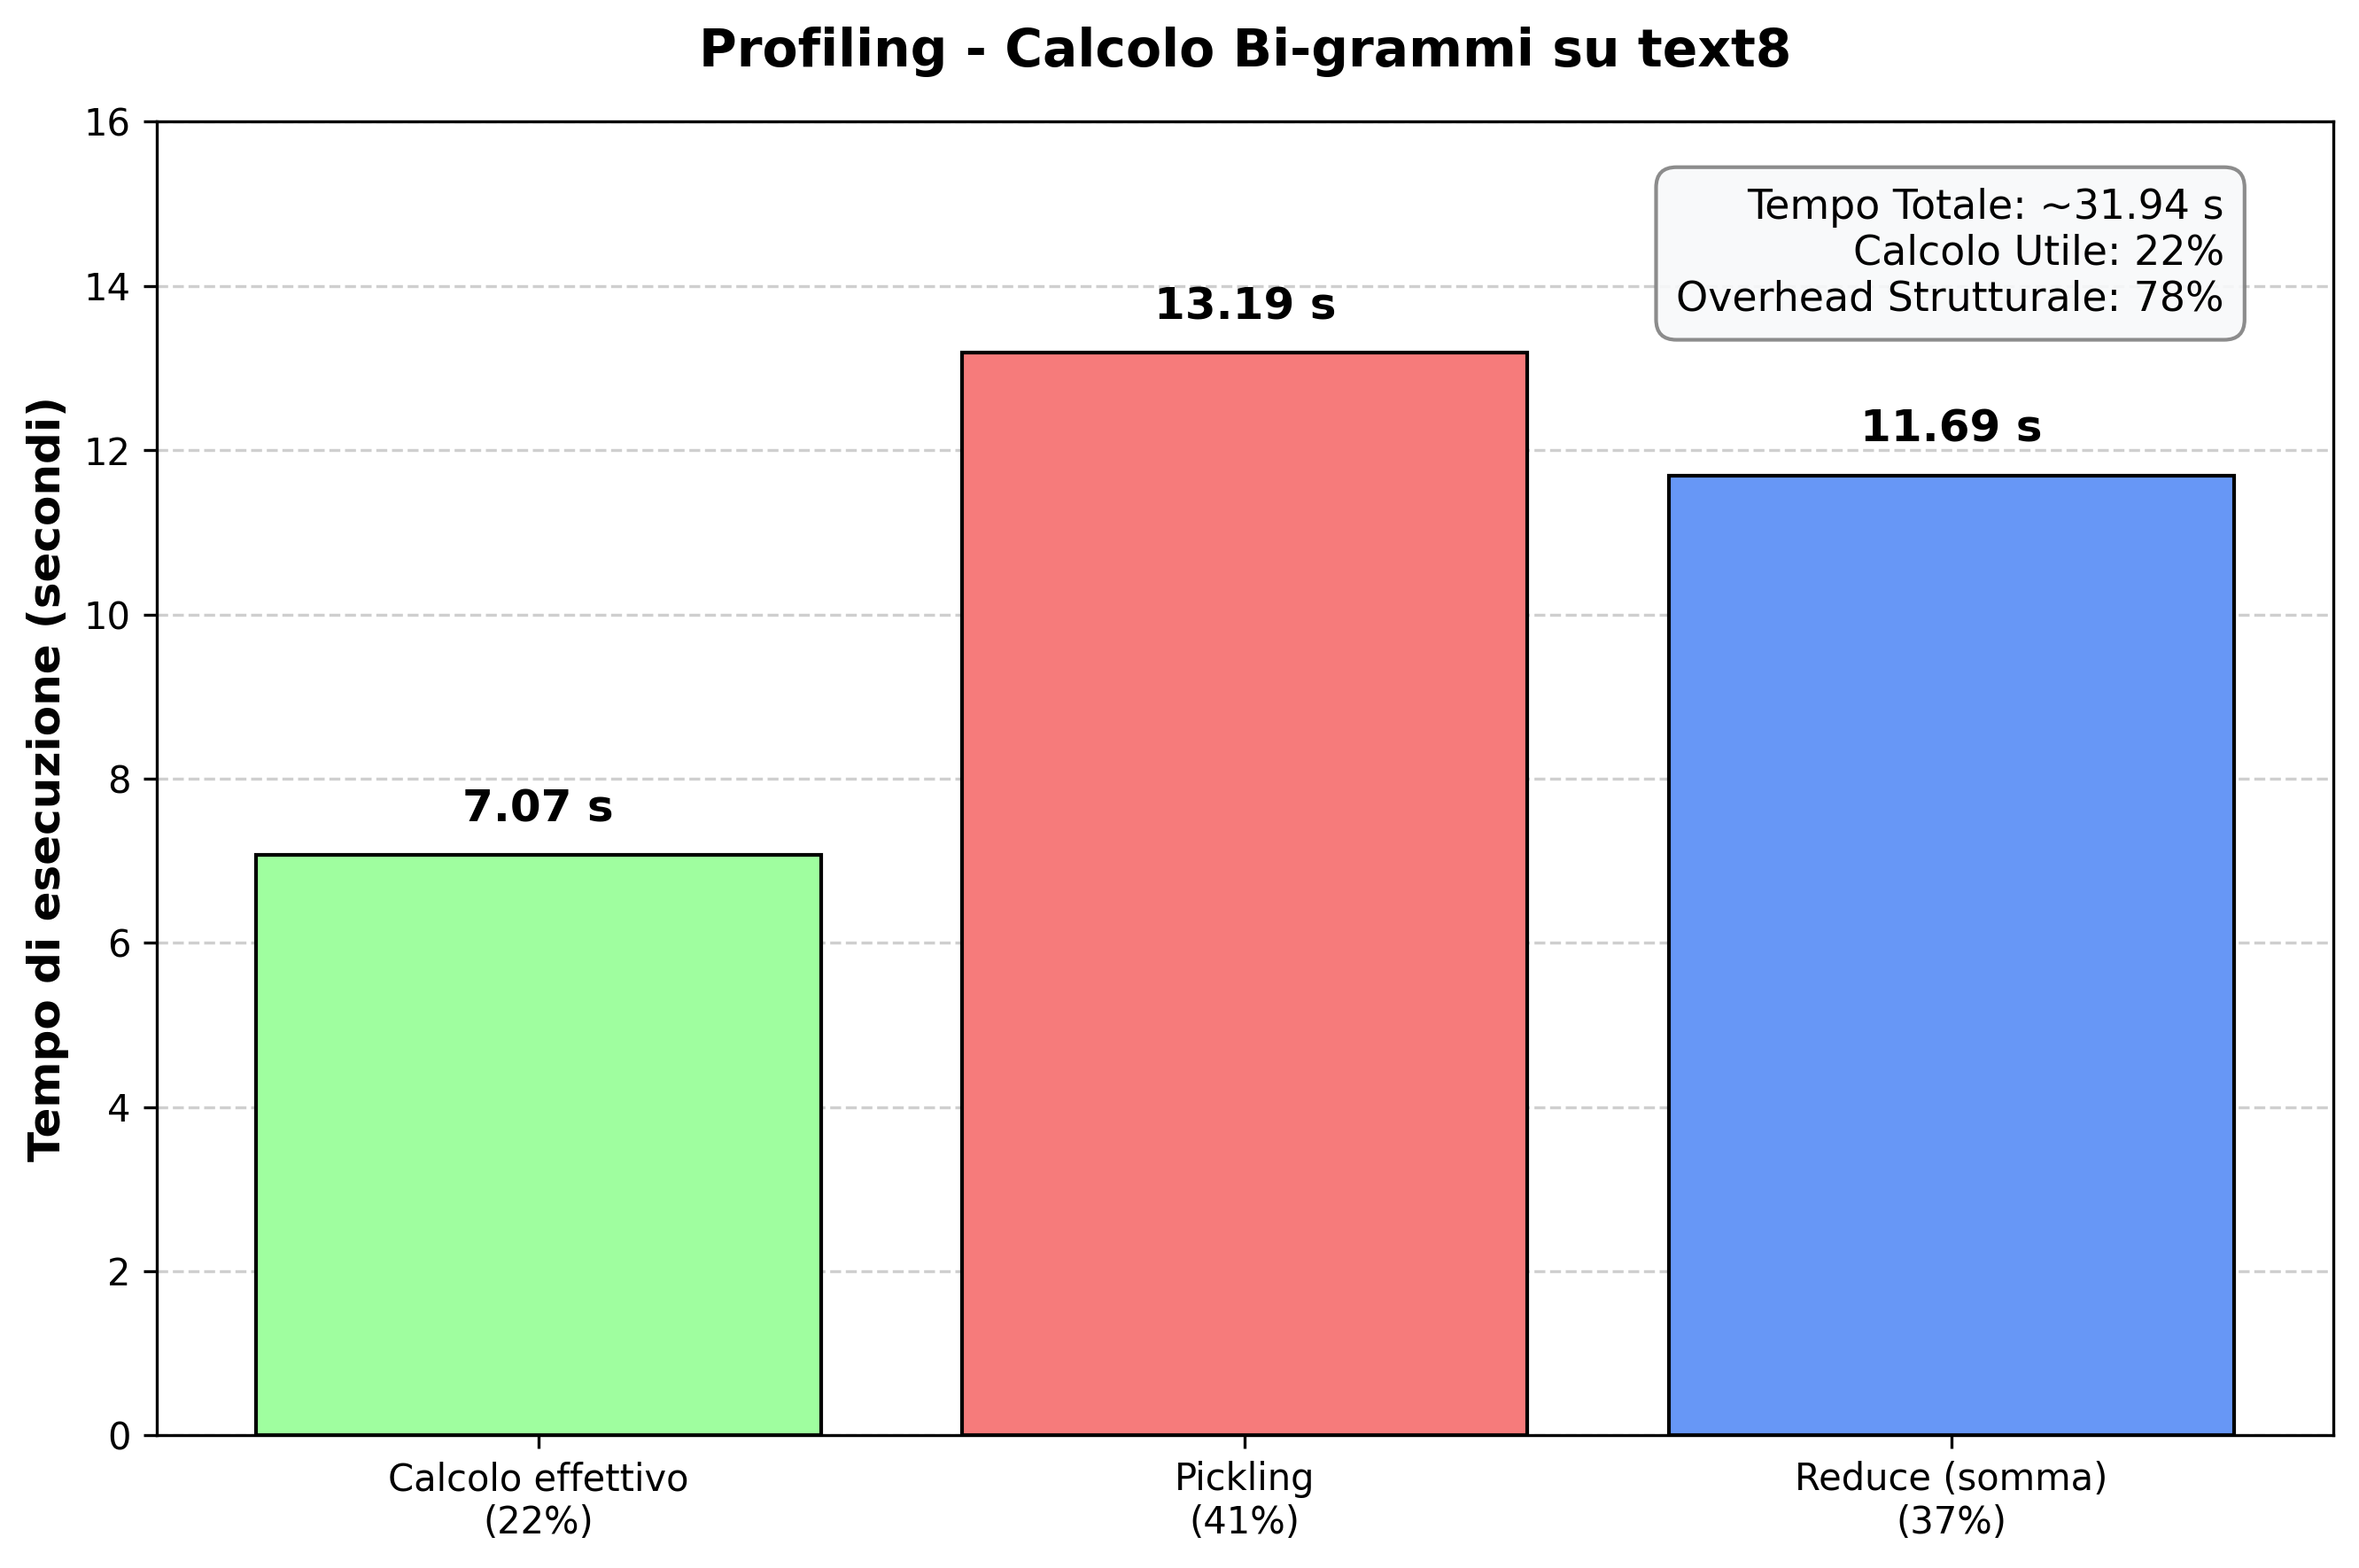
\includegraphics[width=0.9\linewidth]{grafico_profiling_text8.png}
\end{center}
   \caption{Profiling nel calcolo dei bi-gram di parole nel dataset \textit{text8}.}
\label{fig:profiling1}
\end{figure}

Come è possibile vedere il calcolo effettivo, ovvero il conteggio del numero di occorrenze effettuato da ogni processo, impiega solo 7.07 secondi, che rappresenta il 22\% del tempo totale. Da notare che le inefficienze riscontrate con gli n-grams di parole svaniscono nel caso dei caratteri. Questo perchè, mentre il vocabolario di parole può crescere indefinitamente, il vocabolario dei caratteri è finito e di dimensione ristretta, infatti il numero di bigrammi massimo sarà $26^2=676$ e quello dei trigrammi $26^3=17576$.
Questo dimostra chiaramente che per task memory-bound i costi dei trasferimenti dati in memoria annullano totalmente i benefici ottenuti dalla parallelizzazione.


\subsection{Scalabilità}
Valutiamo adesso le versione \textit{Multiprocessing}, sullo stesso task svolto in precedenza, ma stavolta all'aumentare del numero di core utilizzati. Questo ci permetterà di valutare la configurazione ottimale con cui andare a fare il prossimo esperimento. Andiamo quindi a mostrare tempi di esecuzione e speedup ottenuto sul dataset \textit{Frankestein-x50}

\begin{figure}[t]
\begin{center}
   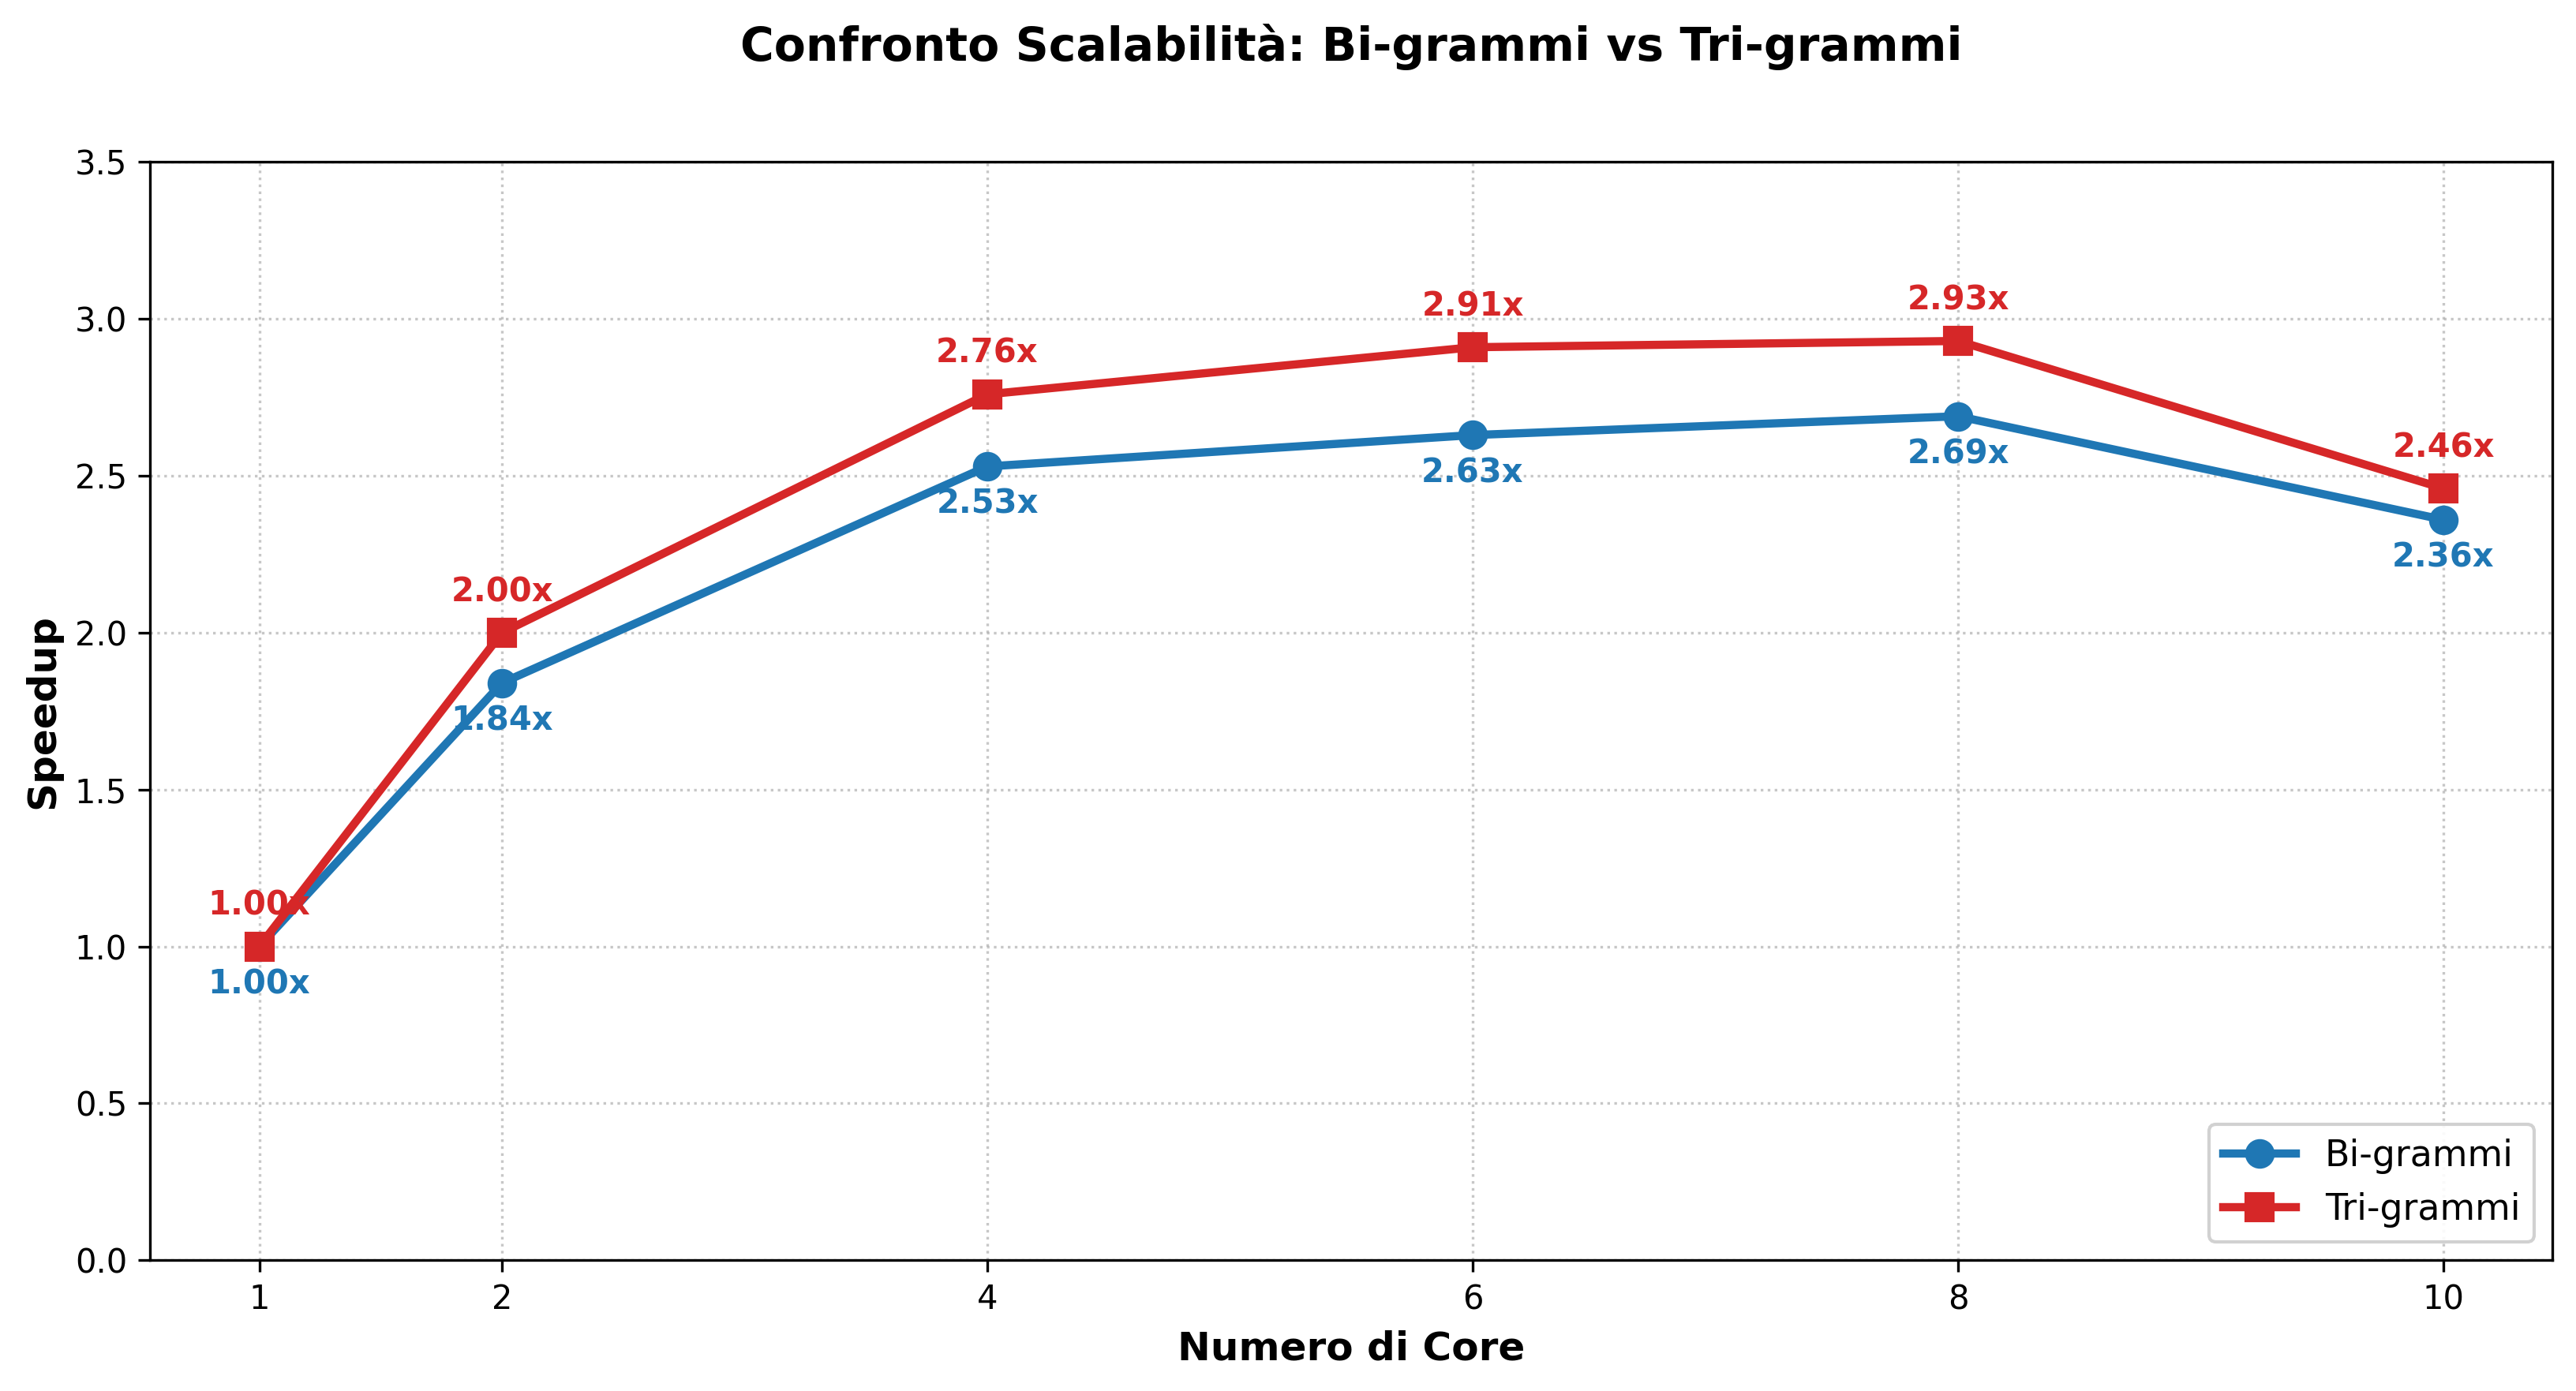
\includegraphics[width=0.9\linewidth]{speed_up_text2.png}
\end{center}
   \caption{Speed-up al variare del numero di core sul Dataset \textit{Frankestein-x50} .}
\label{fig:speeduptext2}
\end{figure}

\begin{figure}[t]
\begin{center}
   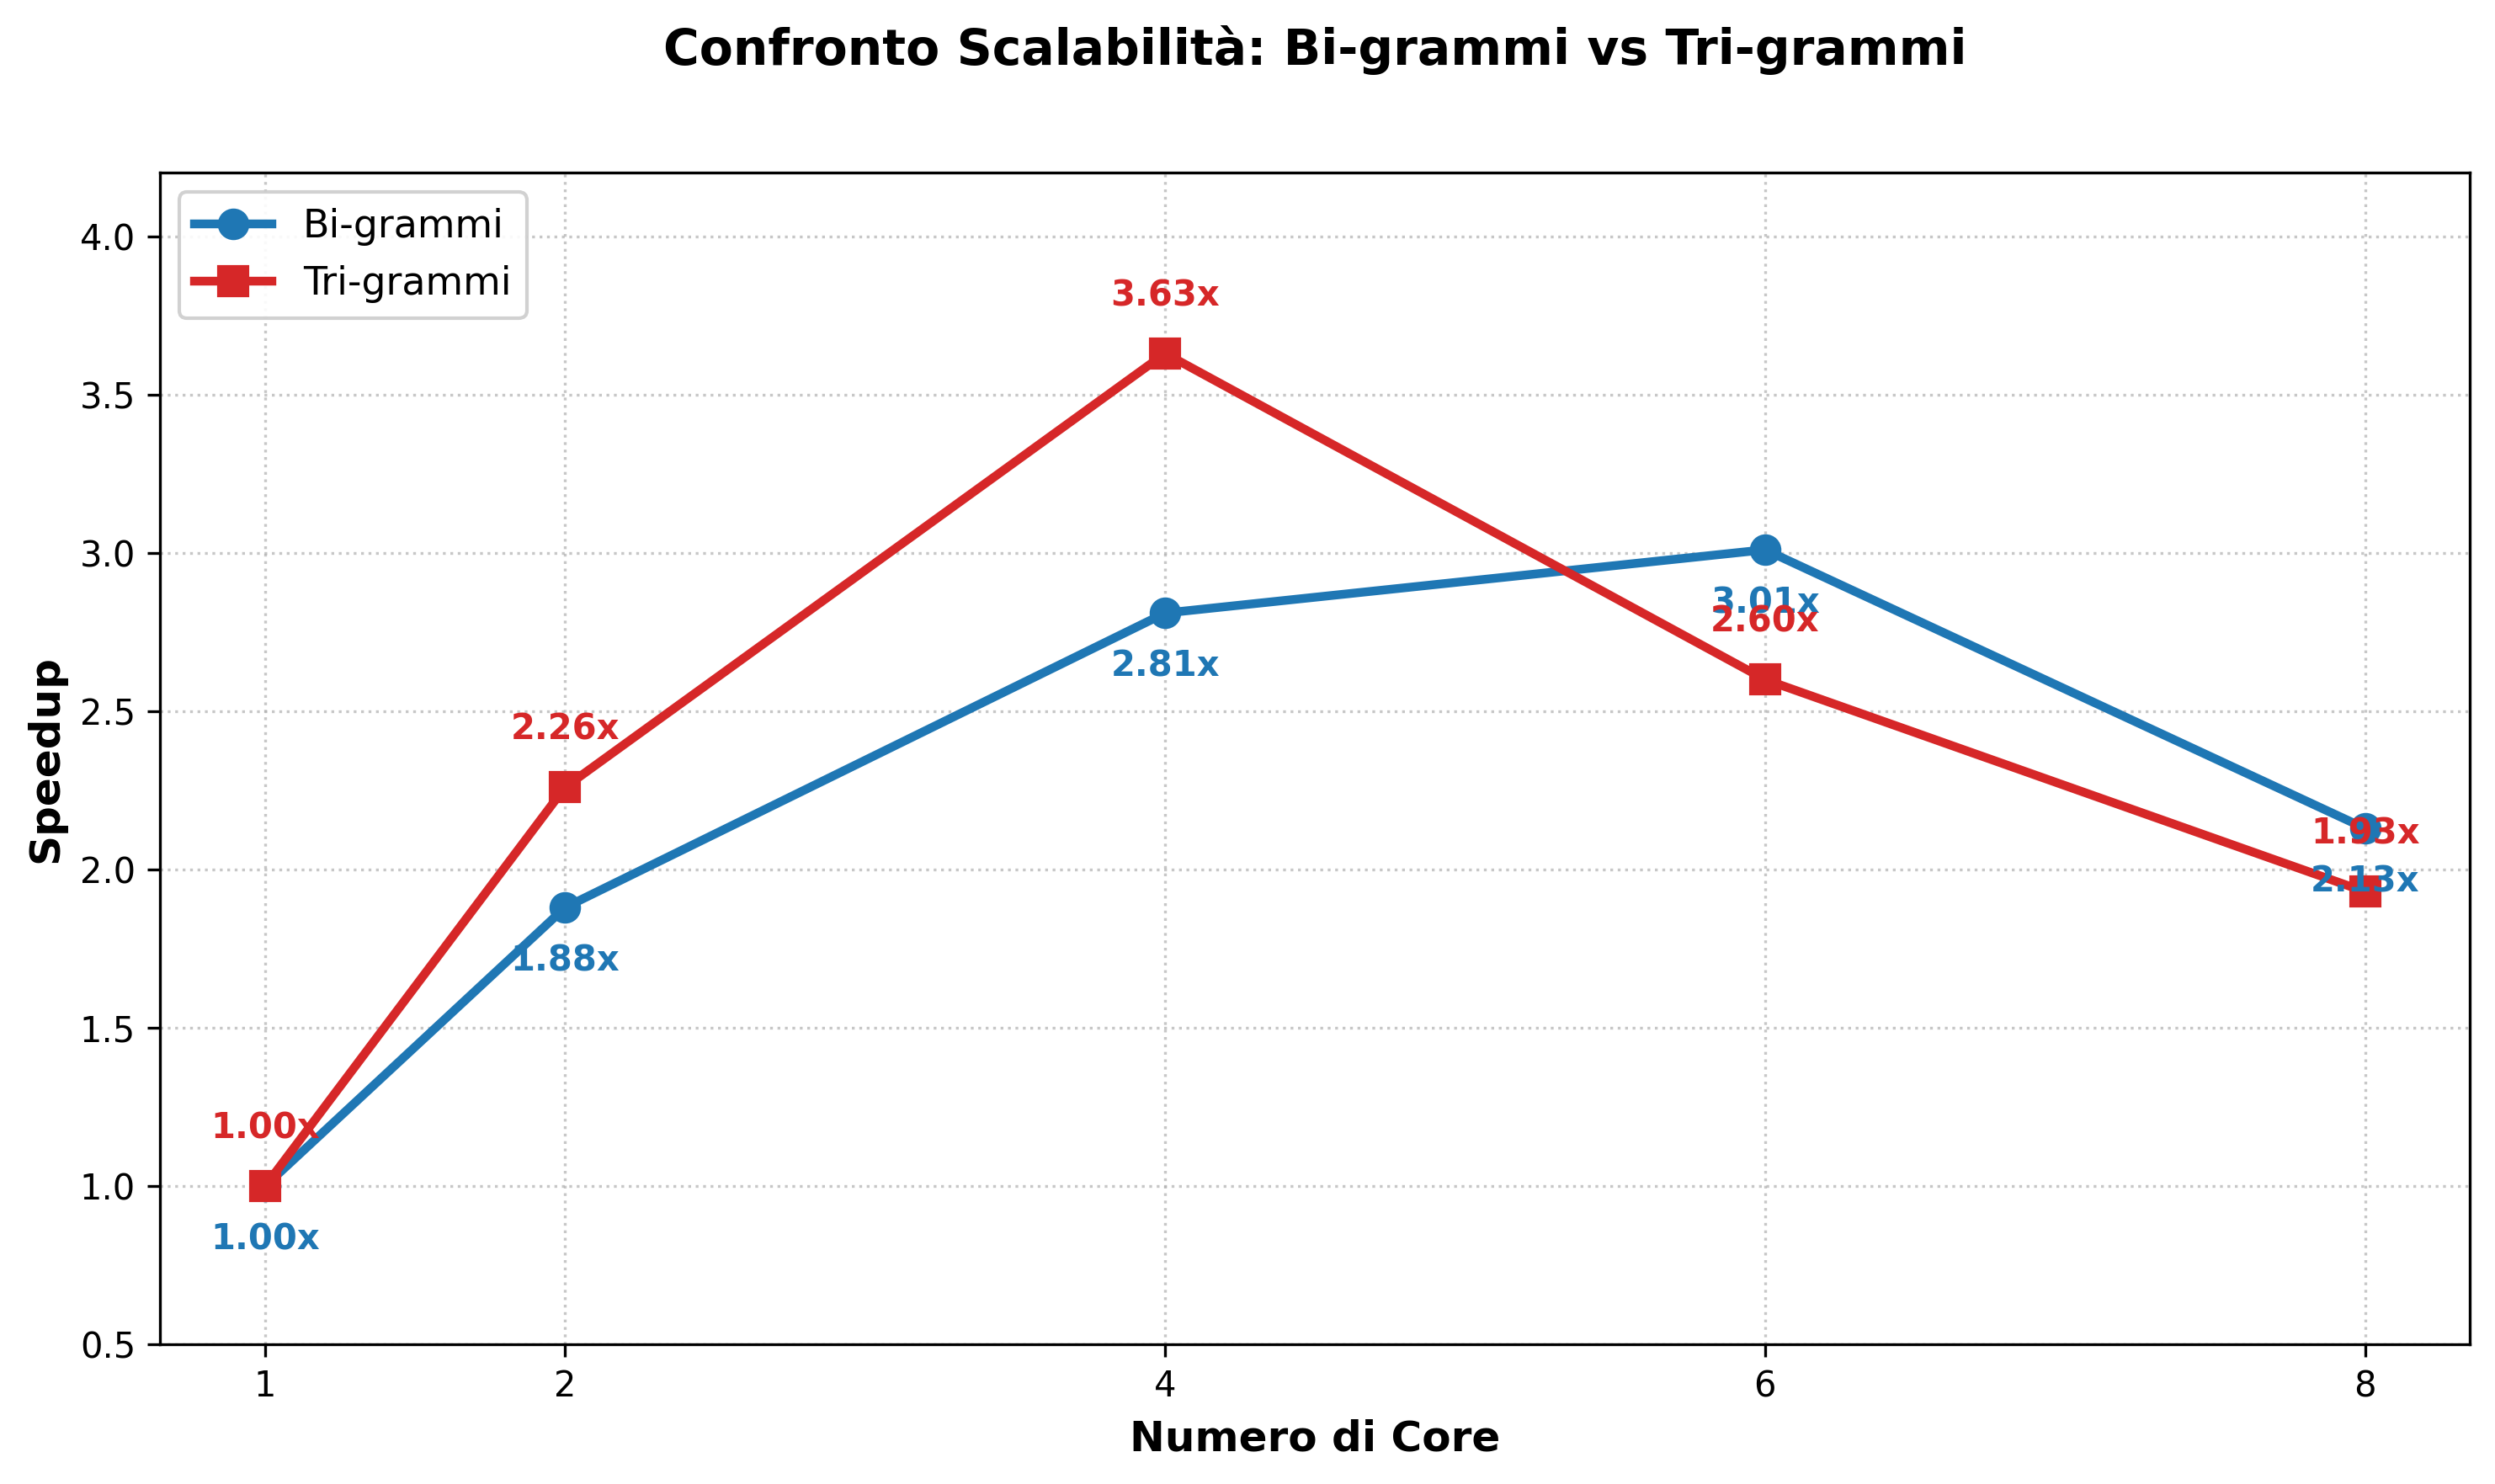
\includegraphics[width=0.9\linewidth]{speed_up_text8.png}
\end{center}
   \caption{Speed-up al variare del numero di core sul Dataset \textit{text8} .}
\label{fig:speeduptext8}
\end{figure}

Possiamo notare nel grafico come per \textit{Multiprocessing} le migliori performance si ottengano con 8 core sia nel caso dei bi-gram, che in quello dei tri-gram. Infatti se aumentiamo ulteriormente i valori di questo parametro, otteniamo risultati che non migliorano, raggiungendo il limite teorico imposto dalla Legge di Amdahl.\par
E' interessante anche il confronto della scalabilità sul dataset \textit{text8} per quanto riguarda il conteggio degli n-gram di caratteri. In questo caso, infatti vediamo un andamento molto più marcato, con un picco nella prestazioni in corrispondenza di 4 core, e successivamente un decremento molto rapido, dovuto probabilmente alla difficoltà di suddividere il testo fra processsi diversi, ma soprattutto alla fase di reduce, che fa sommare dizionari di dimensioni molto più grandi rispetto al dataset \textit{Frankenstein-x50}.





\subsection{Load Balancing}
Procediamo ora con un esperimento che avvicina l'esperimento a quanto viene fatto solitamente nell'ambito del Natural Language Processing. Finora infatti abbiamo diviso in chunk in modo che avessero tutti uguale dimensione; nella realtà invece, spesso il testo viene diviso per capitoli o paragrafi che possono avere lunghezze diverse. Per questo andiamo a modificare la funzione \lstinline{get_chunks} in modo che suddivida i chunk del testo in modo asimmetrico. In particolare andremo a creare appositamente una situazione fortemente sbilanciata, dove i primi K chunk contengono l'80\% del testo, mentre gli altri N-K contengono il restante 20\%.
Multiprocessing andrà quindi a dividere la lista dei task in blocchi di dimensione fissa, assegnando ogni task ad un core in modo casuale. Così facendo un worker può ottenere un blocco che contiene più chunk di dimensione grande, rendendolo così occupato per un tempo elevato.
La libreria Joblib risolve questo problema utilizzando il parametro "batch\_size=auto", che attraverso un'euristica, assegna i task in modo dinamico a ogni worker.
Il risultato è che nei casi in cui a un worker vengono assegnati più task di dimensione elevata questo potrà avere un overtime, dove gli altri processi non avranno nessun calcolo da effettuare.

In particolare l'esperimento è stato effettuato con K=4 e N=200. E in numerose esecuzioni con il dataset \textit{Frankenstein-x50} il codice scrito con \textit{Multiprocessing} aveva questo problema, portando all'assegnazione di almeno due chunk grandi a uno stesso core e un conseguente aumento di tempo, fino al 31\% rispetto a \textit{JobLib}, che invece non presenta mai queata problematica. E' bene dire però che nel caso in cui a tutti i core viene assegnato lo stesso numero di chunk grandi, la differenza fra le due versioni è irrisoria.


%-------------------------------------------------------------------------

\section{Conclusioni}
Il progetto ha quindi analizzato l'efficienza dell'operazione di estrazione degli n-grams, facendo un confronto fra versione sequenziale e varie strategie di parallelizzazione.
Alla luce degli esperimenti condotti quindi, emergono le seguenti conclusioni:
\begin{itemize}
   \item L'elaborazione a livello di carattere si è dimostrata un'operazione molto veloce, che ha mostrato il lato positivo della parallelizzazione. Al contrario il conteggio degli n-grams di parole ci ha permesso di notare come, quando il costo di avvio dei processi paralleli supera il tempo stesso di calcolo, la soluzione sequenziale risulti la migliore
   \item Gli esperimenti hanno dimostrato la limitatezza di \textit{Threading}. A causa del GIL infatti, i thread non possono eseguire del vero parallelismo, rendendoli inutili nell'estrazione degli n-grams. 
   \item Nel caso in cui si vadano a creare dei chunk ben bilanciati non si riscontrano grandi differenze di prestazioni fra \textit{Multiprocessing} e \textit{JobLib}.
   \item Nel caso in cui si abbia uno sbilanciamento del quantitativo di dati \textit{JobLib} risulta essere la scelta migliore, grazie a una miglior gestione dinamica del carico.
\end{itemize}
%-------------------------------------------------------------------------

\section{Specifiche della macchina}

\begin{itemize}
   \item Processore 11th Gen Intel(R) Core(TM) i5-1135G7 @ 2.40GHz 2.42 GHz
   \item RAM installata 8,00 GB (7,70 GB utilizzabile)
   \item Sistema operativo Windows 11 a 64 bit, processore basato su x64
   \item Ambiente di sviluppo: Visual Studio Code
\end{itemize}




\end{document}
